% Four-page main text; references start on a separate page.
\documentclass{l4dc2026}
\usepackage{times}
\usepackage{flafter}
\usepackage{tikz}
\usetikzlibrary{arrows.meta}
\hypersetup{pdftitle={Evaluation-Guided Domain Randomization: Midterm Report},
  pdfauthor={Shimin Chen}}
\title[Evaluation-Guided Domain Randomization]{Evaluation-Guided Domain Randomization:\newline
  Certificates, Controller Updates, and Coverage}
\author{\Name{Shimin Chen} \Email{cshimin@engineering.upenn.edu}}
\makeatletter
\g@addto@macro\ps@jmlrtps{\def\@oddhead{}\let\@evenhead\@oddhead}
\makeatother
\newcommand{\Lhat}{\widehat L_{N,K}}
\newcommand{\Dcert}{\mathcal D_{\mathrm{cert}}}
\newcommand{\Pclass}{\mathcal P}
\newcommand{\G}{G_K}
\begin{document}
\maketitle
\begin{abstract}
Can boundary-targeted training enlarge a controller's acceptable operating
conditions? We connect trajectory-based certificate learning to a safe
linear-controller update, with an elementary generalization proof, a
stability-preserving update, and a numerical study of how its components interact.
The chosen certificate sets how far each update can go, while the training target
matters only when plants disagree. Our main goal is now to prove when an update
enlarges coverage.
\end{abstract}

\section{Question, feedback loop, and setting}
Domain randomization trains one controller across varying plants and initial
conditions. We ask whether evaluation can guide it: if training emphasizes conditions
near the boundary of acceptable performance, does the set of acceptable conditions
grow? Each outer round $k$ closes the loop
\[
 \underbrace{K_k}_{\text{controller}}
 \longrightarrow
 \underbrace{\tau_{K_k}}_{\text{trajectories}}
 \longrightarrow
 \left\{\begin{array}{l}
  \text{evaluate costs, choose training distribution } q_k\\
  \text{fit, then verify, certificate } P_k
 \end{array}\right\}
 \longrightarrow
 \underbrace{K_{k+1}}_{\text{safe update}}
\]
State feedback closes the inner loop within each trajectory; $P_k$ may be fixed or
refitted.

\textbf{Why this is an L4DC problem.}
The controller being improved also generates the data used to judge it. Changing
$K$ changes the closed-loop trajectories, so a certificate fitted to old
trajectories carries no statistical guarantee for the new controller, and the
acceptance boundary moves. We therefore separate what needs fresh trajectories from
what an update can preserve deterministically.
We adapt the continuous-time framework of
\citet[Sections~3--4]{boffi2021learning} to discrete time; starting-state
curricula \citep{florensa2017reverse} motivate boundary targeting.

\textbf{Progress since the proposal.}
We proved the bound and verification test of Section~\ref{sec:approach} (full proofs
are in our research note), implemented the safe update, and measured how refitting,
targets, and plant families interact, and ran the loop on CartPole with PPO. Proofs of the cost-drift bound and small-step acceptance are in draft.

\textbf{Plants, conditions, and trajectories.}
Let $\theta\in\Theta$ index a finite known plant family. State $x_t\in\mathbb R^n$
and input $u_t\in\mathbb R^m$ evolve under a shared gain $K\in\mathbb R^{m\times n}$:
\begin{equation}\label{eq:mid_dynamics}
 x_{t+1}=A(\theta)x_t+B(\theta)u_t=\G(\theta)x_t,
 \quad u_t=-Kx_t,\quad \G(\theta)=A(\theta)-B(\theta)K.
\end{equation}
Dynamics are deterministic, fully observed, and unconstrained. A \emph{condition} $z=(\theta,x_0)$ pairs a plant with a reset in
$\mathcal X_0=\{x:\|x\|_2\le r_0\}$, with radius $r_0>0$. Its trajectory
$\tau_K(z)=(x_0,\ldots,x_H)$ has $H$ transitions of that one plant.
Matrix norms $\|\cdot\|_2$ and $\|\cdot\|_F$ are operator and Frobenius.

\textbf{Performance.}
Fix state-cost weight $Q\succeq0$, input-cost weight $R\succ0$, cost threshold
$h>0$, and evaluation distribution $\mu$ on $\Theta\times\mathcal X_0$, which
weights conditions when measuring overall performance and never changes. The
trajectory cost, acceptable set, and coverage (acceptable fraction) are
\begin{equation}\label{eq:mid_cost}
 J_{H,K}(z)=\sum_{t=0}^{H-1}(x_t^\top Qx_t+u_t^\top Ru_t),\quad
 S_K^J=\{z:J_{H,K}(z)\le h\},\quad C_J(K)=\mu(S_K^J).
\end{equation}

\textbf{Certificate loss}
For the linear plant family, the goal is to fit a Lyapunov certificate
$P\in\Pclass=\{P=P^\top:aI\preceq P\preceq bI\}$, where $0<a<b$ bound the eigenvalues,
whose energy $V_P(x)=x^\top Px$ satisfies, for each $\theta\in\Theta$ and each state $x$
with successor $x^+=\G(\theta)x$, the desired decrease
$V_P(x^+)-V_P(x)\le-\eta\|x\|_2^2$, with $\eta>0$ predeclared. This motivates us to
define the transition-wise residual
$r_P(x,x^+)=(V_P(x^+)-V_P(x))/\|x\|_2^2+\eta$ and subsequently, with predeclared
margin $\gamma>0$, the trajectory-wise worst residual $s_P$ and a surrogate loss $\ell_P$:
\begin{equation}\label{eq:mid_loss}
 s_P(\tau)=\max_{0\le t<H:\,x_t\ne0}r_P(x_t,x_{t+1}),\qquad
 \ell_P(\tau)=\min\{1,\max\{0,1+s_P(\tau)/\gamma\}\}.
\end{equation}
Under these definitions, $r_P\le0$ means the energy decreases by at least
$\eta\|x\|_2^2$ after one transition, and $\ell_P=0$ means the decrease is at least
$(\eta+\gamma)\|x\|_2^2$ throughout the trajectory.\footnote{We skip $x=0$ and set
$\ell_P=0$ for all-zero trajectories.}

Under a frozen $K$ and the certificate-sampling distribution $\Dcert$, we use the
population loss $L_K(P)=\mathbb E_{\Dcert}\,\ell_P(\tau_K(z))$ as the training goal, for
which in practice we minimize the empirical loss
$\Lhat(P)=\frac1N\sum_{i=1}^N\ell_P(\tau_i)$, where $\tau_i$ are the trajectories of $N$
i.i.d.\ conditions.

\section{Solution approach}\label{sec:approach}
\textbf{What generalizes: a uniform bound.}
Let $M_K=\max_{\theta\in\Theta}\|\G(\theta)\|_2$. The loss is Lipschitz in $P$ under
the Frobenius norm, with constant $L_{\mathrm{par}}=(M_K^2+1)/\gamma$.
Before sampling, choose a net resolution $\varepsilon>0$ and failure probability
$\delta\in(0,1)$. A data-independent Frobenius $\varepsilon$-net of $\Pclass$ has at
most $(1+2b\sqrt n/\varepsilon)^d$ centers, where $d=n(n+1)/2$ counts symmetric
parameters. For any $P$, take a center $P_\varepsilon$ within $\varepsilon$. Each arrow
bounds an absolute difference:
\begin{center}
\vspace{-5pt}
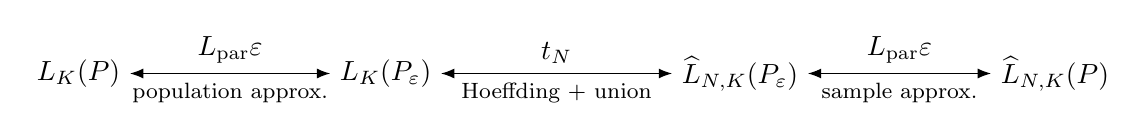
\begin{tikzpicture}[>=Latex,baseline]
 \node (a) at (0,0) {$L_K(P)$};
 \node (b) at (3.9,0) {$L_K(P_\varepsilon)$};
 \node (c) at (8.4,0) {$\Lhat(P_\varepsilon)$};
 \node (d) at (12.4,0) {$\Lhat(P)$};
 \draw[<->] (a) -- node[above] {$L_{\mathrm{par}}\varepsilon$}
   node[below,font=\footnotesize] {population approx.} (b);
 \draw[<->] (b) -- node[above] {$t_N$}
   node[below,font=\footnotesize] {Hoeffding + union} (c);
 \draw[<->] (c) -- node[above] {$L_{\mathrm{par}}\varepsilon$}
   node[below,font=\footnotesize] {sample approx.} (d);
\end{tikzpicture}
\vspace{-5pt}
\end{center}
The union bound makes the middle arrow hold for all centers at once, and the triangle
inequality adds the three, paying approximation twice. Thus, with probability at least
$1-\delta$, for every $P\in\Pclass$,
\[
 |L_K(P)-\Lhat(P)|\le\Delta_N=2L_{\mathrm{par}}\varepsilon+t_N,
 \quad\text{where}\quad
 t_N=\sqrt{\frac{d\log(1+2b\sqrt n/\varepsilon)+\log(2/\delta)}{2N}}.
\]
This simultaneous bound also covers a matrix $\widehat P$ fitted on the same data.
Since $s_P(\tau)>0$ forces $\ell_P(\tau)=1$, it also limits the violation probability on a
fresh condition: $\Pr_{\Dcert}\{s_{\widehat P}(\tau_K(z))>0\}\le\Lhat(\widehat P)+\Delta_N$.
The bound applies only to frozen
$K$ and trajectories from $\Dcert$, so each new controller needs fresh trajectories,
and it does not reproduce Boffi et al.'s faster rates.

\textbf{What verifies stability: a deterministic test.}
Low violation probability implies neither stability nor the desired decrease, so the
update uses a deterministic test, not the bound. For a declared nonempty retention set
$\Theta_{\mathrm{ret}}\subseteq\Theta$, the verified decrease margin is
$\eta_\theta(P)=\lambda_{\min}(P-\G(\theta)^\top P\G(\theta))$, and $P$ is \emph{verified}
at $K$ if this is positive on that set. All retained fixed-plant loops are then globally
exponentially stable under one shared $V_P$, a restriction beyond stability of each plant, and
$\eta_\theta(P)\ge\eta$ gives the desired decrease everywhere.

\textbf{Safe means stable \citep{berkenkamp2017safe}.}
To keep $P$ verified when $K$ becomes $K^+=K+\Delta K$, we start from this margin and bound
how much the step can lower it. The closed loop $G=\G(\theta)$ becomes $G+E$, with
$E=-B(\theta)\Delta K$ and $d_\theta=\|E\|_2$. Expanding $(G+E)^\top P(G+E)$ shows that the
margin of the same $P$ at $K^+$ satisfies $\eta_\theta^+(P)\ge\eta_\theta(P)-c_\theta(\Delta K)$, where
$c_\theta(\Delta K)=2\|G^\top P\|_2d_\theta+\|P\|_2d_\theta^2$ bounds the terms in $E$. To
retain a fraction $\rho\in(0,1)$ of the margin, the \emph{safety test} requires
$c_\theta(\Delta K)\le(1-\rho)\eta_\theta(P)$ on the retention set, so
$\eta_\theta^+(P)\ge\rho\eta_\theta(P)>0$. With this test, $P$ stays verified at $K^+$,
and the next round can start from it. Keeping $\eta$ also requires $\rho\eta_\theta(P)\ge\eta$. The test also requires $\|\Delta K\|_2\le\kappa$, $\kappa>0$,
for cost bounds, not stability.

\textbf{What is new: evaluation-guided targeting.}
This is our main novelty. By iterating certificate learning after
\citet{boffi2021learning} and domain-randomized control after
\citet{fujinami2025domain}, we seek to generate controllers and certificates while
requiring only finite-horizon rollouts. Fujinami et al.\ weight plants uniformly or
toward high cost; we target the acceptance boundary. Keep $\mu$ fixed and adapt a
training distribution $q$ on a finite condition grid $\mathcal Z$: target $q_{\mathrm{tar}}$
restricts a positive background $q_{\mathrm{base}}$ to the \emph{boundary band}
$|J_{H,K}-h|\le w$, $w>0$, and normalizes it (background if empty), and for
$\lambda\in[0,1)$, $q=(1-\lambda)q_{\mathrm{base}}+\lambda q_{\mathrm{tar}}$. The objective
is $F_q(\widetilde K)=\sum_{z\in\mathcal Z}q(z)J_{H,\widetilde K}(z)$.

\begin{algorithm2e}[H]
\small
\DontPrintSemicolon
\SetAlgoNoEnd
\SetCommentSty{textit}
\SetKwComment{Comment}{$\triangleright$ }{}
\caption{One safe Armijo update \citep{armijo1966minimization}: one round of the loop.}
\label{alg:mid_update}
\KwIn{Gain $K$; $P$ verified at $K$, kept or refitted; maximum step $s_0>0$; $\beta,c_A\in(0,1)$; $J_{\max}\ge0$.}
Roll out $K$ on $\mathcal Z$, build $q$ from the costs $J_{H,K}(z)$, and freeze it\Comment*[r]{data only}
Compute $D=-\nabla_KF_q(K)$; if $D=0$, \Return{$K$}\Comment*[r]{exact; this and the safety test use known plants}
Set $\bar s=\min\{s_0,\text{\emph{step capacity} of }P\text{ along }D\}$\Comment*[r]{largest $s$ for which $sD$ passes the safety test}
\For(\Comment*[f]{shrink by $\beta$, not a fixed step grid; every trial passes the test}){$s=\bar s\beta^j$, $j=0,\ldots,J_{\max}$}{
 \lIf{$F_q(K+sD)\le F_q(K)-c_As\|D\|_F^2$}{\Return{$K+sD$}\hfill\Comment*[h]{Armijo condition, coefficient $c_A$}}
}
\Return{$K$}\Comment*[r]{strict margins and smooth costs: an uncapped search succeeds}
\end{algorithm2e}

\noindent\emph{Safe descent need not preserve coverage:} with hand-set $q$, in a two-plant scalar
example an accepted step lowers $F_q$ and keeps margins positive, yet coverage halves (boundary
targeting gives $D=0$).

\section{Preliminary results}\label{sec:results}
Experiments check the statements above and measure how components interact. Two-plant linear families run the update of Section~\ref{sec:approach} for
three rounds from the same starting coverage. Four family types differ in how much their
plants disagree: same-shape (similar plants), random stable pairs, random pairs with a
rotated second actuator, and mirrored pairs ($G_2\approx-G_1$). We fit $P$ by exhaustive
search over a fixed grid of 874 matrices, taking the first empirical minimizer in grid
order. Every family runs every combination of refitting and target.

\begin{figure}[t]
 \centering
 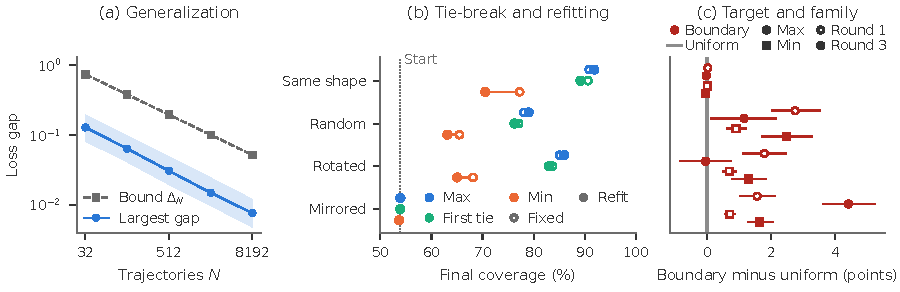
\includegraphics[width=\linewidth]{midterm_assets/linear_results.pdf}
 \vspace{-8pt}
 \caption{(a) Median largest loss gap and 10th--90th dataset percentiles, with a risk
 floor added. (b) Mean coverage under background targeting. (c) Mean gain of boundary over uniform
 background (grey line), fixed $P$, 95\% intervals.}
 \label{fig:mid_results}
 \vspace{-22pt}
\end{figure}

\textbf{The bound holds.}
In Figure~\ref{fig:mid_results}(a) the gap stays below $\Delta_N$, and both shrink like
$1/\sqrt N$.

\textbf{Refitting.}
Refitting $P$ at each updated $K$ is a natural next step, since the bound holds only
for a frozen $K$ and a new controller needs fresh trajectories anyway. We tried this,
drawing fresh trajectories each round and verifying the new $P$ before using it. In
Figure~\ref{fig:mid_results}(b), final coverage barely moves: it falls by at most
1.5 points on three families and is unchanged on mirrored plants. A rule that favors
step capacity reverses this by about 1 point. The theory allows this: verification and the safety test hold for
whichever verified $P$ is in use, but each round then has its own certificate rather
than one $V_P$ shared across rounds. A new $P$ changes the safety test, not $D$, so it
acts only through the step it permits, and fitting ignores that step.

\textbf{Targets and families.}
We compared boundary targeting against the uniform background across the four plant
families. Figure~\ref{fig:mid_results}(c) shows that its benefit depends on how much
the plants disagree. It has no effect on same-shape plants. On random and rotated
plants it leads by about 2 points after one round, but that lead is no longer
distinguishable from zero by round 3. On mirrored plants its lead grows to about
4 points, because background targeting trades gains for losses and makes no net
progress. This can be explained by what the safety test limits: it bounds $\Delta K$,
not $s$, so when it sets the step, a target acts only by turning $D$, which requires
plants that disagree. About a third of random and rotated pairs have no shared
certificate on our grid and are left out of these means.

\textbf{CartPole with PPO (development pilot).}
With no certificate, we ran the loop from a frozen PPO policy: evaluate recovery
across initial angle and pole length, refresh the frontier, retrain. On held-out
evaluations through 153,600 transitions (Figure~\ref{fig:ppo_loop}), the accepted set
about doubles in all three seeds, while 6--15 of the parent's 28 conditions are lost.
Later rounds drift to shorter poles and lose nominal recovery, so larger coverage need
not mean retained competence.

\begin{figure}[!h]
 \centering
 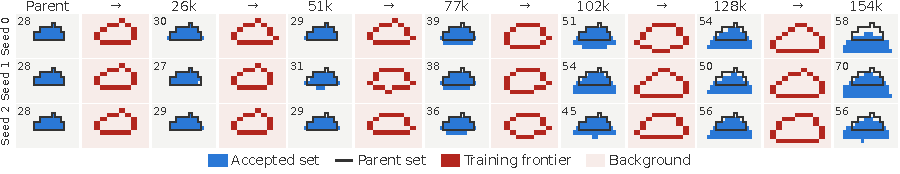
\includegraphics[width=\linewidth]{midterm_assets/ppo_loop.pdf}
 \vspace{-8pt}
 \caption{Interleaved loop, left to right: each held-out accepted set (recovery rate at
 least 0.9) precedes the frontier for the next 25,600 transitions. Axes: angle, pole length.}
 \label{fig:ppo_loop}
 \vspace{-26pt}
\end{figure}

\section{Challenges and remaining work}
\textbf{Challenges.}
\emph{A conservative, sign-blind safety test:} it charges worst-case margin use even when an
update raises the margin, so step capacity can fall far below what stability needs.
\emph{A vacuous cost-drift bound:} only conditions within the largest possible cost change
$b_J(\theta)$ below $h$ can be lost, so their $\mu$-mass bounds lost coverage, but in our first
test $b_J$ was roughly 50 times the actual change.

\textbf{Remaining work.}
Most remaining effort is theoretical: (1) finish the update proofs; (2) prove a
coverage lower bound computable before updated costs are observed, from a second-order
upper envelope of each cost along $D$; (3) find assumptions that make it positive, through
gradient alignment, conflict, and the step needed to cross $h$; (4) tighten curvature
bounds, make that test sign-aware, and prove how refitting acts through
step capacity. Experiments then test it.

\noindent\textit{AI assistance:} Codex \& Claude assisted with drafting and preliminary derivations.
\label{midterm_body_end}

\clearpage
\label{midterm_references_start}
\bibliography{references.bib}
\end{document}
